\chapter{Estado del arte} \label{estado_del_arte}

\section{Análisis de las posibles soluciones al problema propuesto}
La gestión completa de pisos compartidos siguiendo los principios de convivencia propuestos por el \emph{co-housing}  plantea diversos desafíos, donde la tecnología puede ofrecer una solución efectiva que facilite su implementación.

En este contexto, es fundamental analizar y entender las soluciones tecnológicas existentes en el mercado, analizando tanto su enfoque como las herramientas utilizadas.

Para la realización de este estudio, se han analizado distintos proyectos y aplicaciones con el objetivo de identificar soluciones propuestas con anterioridad a este problema, se ha hecho especial enfoque en la usabilidad y en las herramientas utilizadas, tratando de extraer las mejores prácticas que sirvan de referencia para la creación de una solución efectiva.

\section{Revisión del estado del arte}
Para la realización de la revisión se va a seguir un esquema de temáticas, el proyecto se sustenta en dos grandes bloques: la gestion de tareas en viviendas compartidas y la búsqueda de pisos en función de afinidad entre personas. Dentro de estas dos temáticas será donde se analizarán las soluciones existentes,  buscando su aportación al enfoque de co-housing en pisos compartidos.


\subsection{Búsqueda de pisos}
\subsubsection{Idealista}
    \emph{Idealista}\cite{Idealista} es un portal inmobiliario que permite la búsqueda de pisos y habitaciones en función de criterios como la ubicación, rango de precio, aceptación de fumadores y predisposición a mascostas. Es un portal ampliamente usado, por lo que contiene un gran volumen de ofertas en distintas ciudades.
    Sin embargo, no incorpora ninguna funcionalidad que permita evaluar la afinidad entre posibles inquilinos en función de sus intereses o estilo de vida. 

\begin{figure}[H]
    \centering
    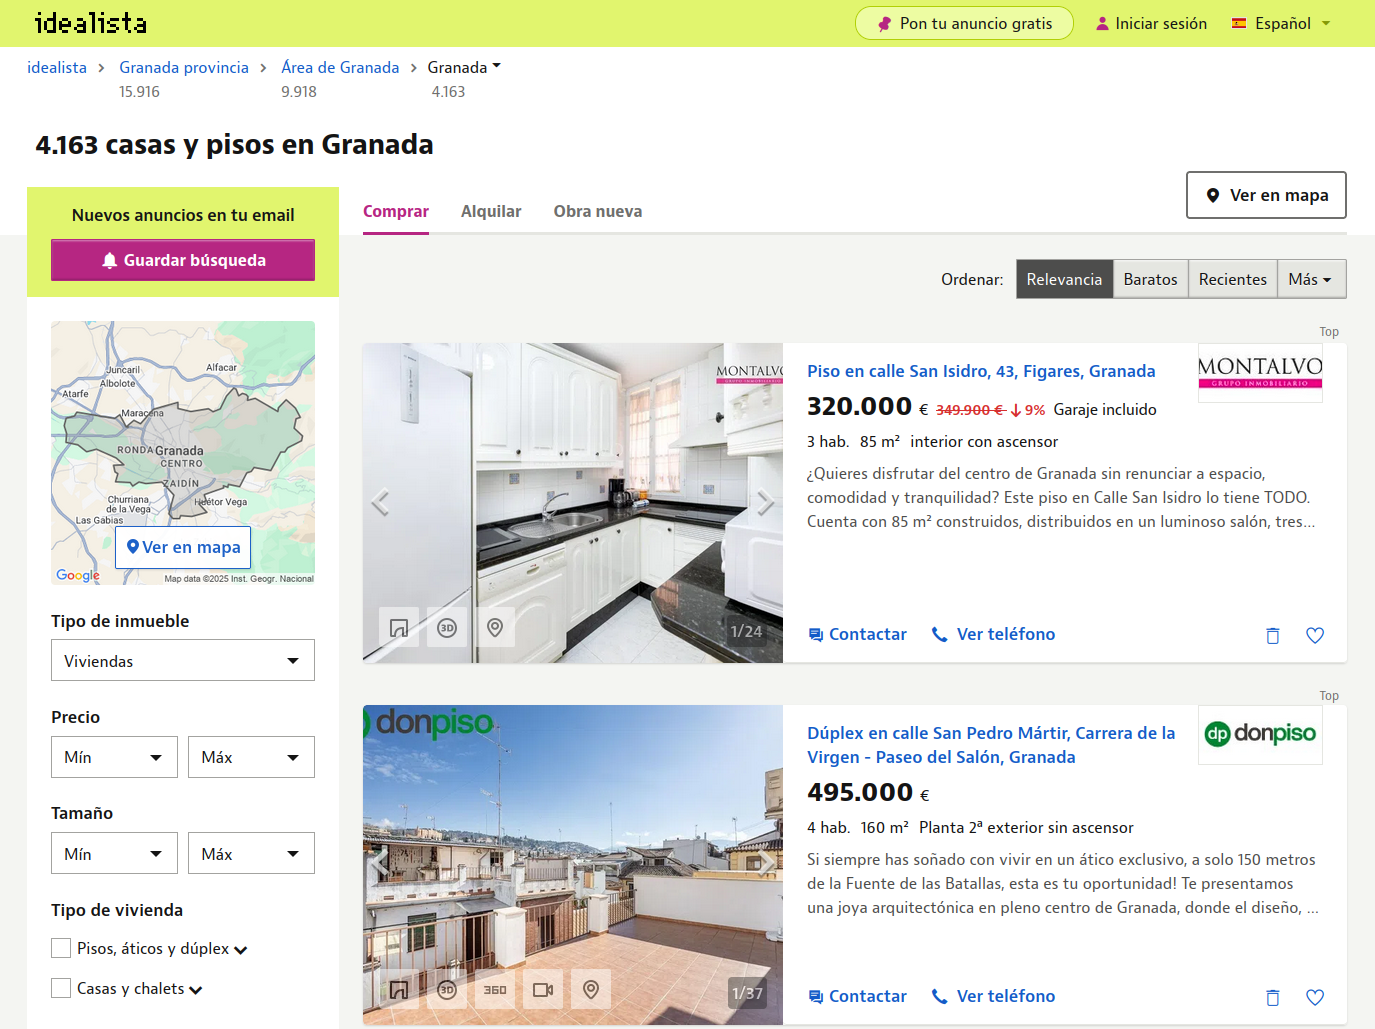
\includegraphics[width=0.8\textwidth]{fotos/idealista.png}
    \caption{Interfaz de búsqueda de Idealista\textbf{}.}
    \label{fig:idealista}
\end{figure}

\subsubsection*{Interfaz y usabilidad}
Como se puede ver en la imagen \ref{fig:idealista}, la interfaz es simple e intuitiva lo que permite que se entienda toda su funcionalidad a la perfección. Es de destacar que la aplicación te permite, con pocas configuraciones, empezar la búsqueda de piso por lo que se hace muy cómoda de usar.

\subsubsection*{Características destacadas}
\begin{itemize}
    \item \textbf{Gran volumen de ofertas:} Al ser una plataforma muy popular cuenta con un gran número de ofertas en distintas ciudades.
    \item \textbf{Filtros de búsqueda:} Permite aplicar una serie de criterios en la búsqueda como rango de precios, aceptación de fumadores, predisposición a mascotas, lo cual ayuda al usuario a encontrar un piso más acorde a sus necesidades
    \item \textbf{Comunicacion cliente-ofertante sencilla:} Facilita con su chat integrado la comunicación entre cliente y ofertante ya sea para consultar alguna duda o para realizar una reserva.
\end{itemize}
\subsubsection*{Limitaciones}
\begin{itemize}
    \item No tiene en cuenta la afinidad entre los inquilinos, lo que puede provocar que personas con diferentes intereses acaben conviviendo juntos.
    \item Se centra únicamente en la oferta de pisos, sin ofrecer ninguna herramienta para gestionar la vivienda compartida.
    \item La aplicación está orientada simplemente a encontrar potenciales inquilinos, ignorando la integración del nuevo miembro en la vivienda.
\end{itemize}

\subsubsection*{Conclusión}
\emph{Idealista} es una buena opción como portal de viviendas, ofrece posibilidades en prácticamente todas las ciudades y su facilidad de uso es correcta. Sin embargo, para la idea que buscamos es incompleta al no ofrecer nada relacionado con la búsqueda por afinidad.

\subsubsection{Flatmate Finders}
\emph{Flatmate Finders} \cite{Flatmatefinders} es una plataforma que ofrece una solución bastante precisa al problema de búsqueda de pisos por afinidad. Permitiendo al usuario dos opciones principales:

\begin{enumerate}[label=\arabic*)]
    \item \textbf{Buscar un piso}: el usuario puede crearse un perfil con información sobre su personalidad, gustos y preferencias. A partir de estos datos, la aplicación genera recomendaciones de ofertas de pisos mostrando un porcentaje de compatibilidad.
    \item \textbf{Ofrecer un piso}: los propietarios pueden registrar su vivienda, estableciendo detalles como ubicación, precio, características y criterios sobre el perfil de los inquilinos afines.
\end{enumerate}
\newpage
\begin{figure}[H]
    \centering
    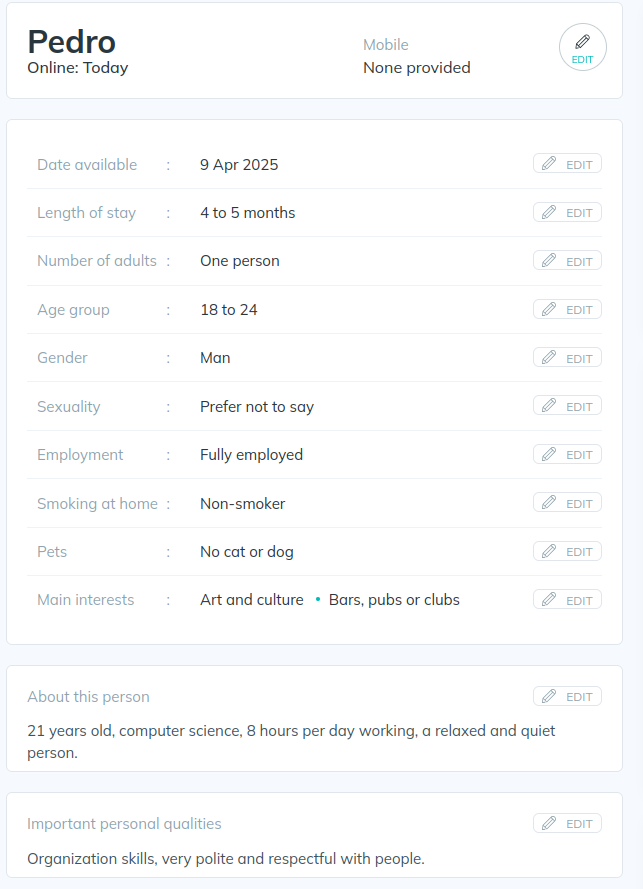
\includegraphics[width=0.8\textwidth]{fotos/perfil-flatmate.png}
    \caption{Configuración del perfil de usuario \textbf{}.}
\end{figure}
\begin{figure}[H]
    \centering
    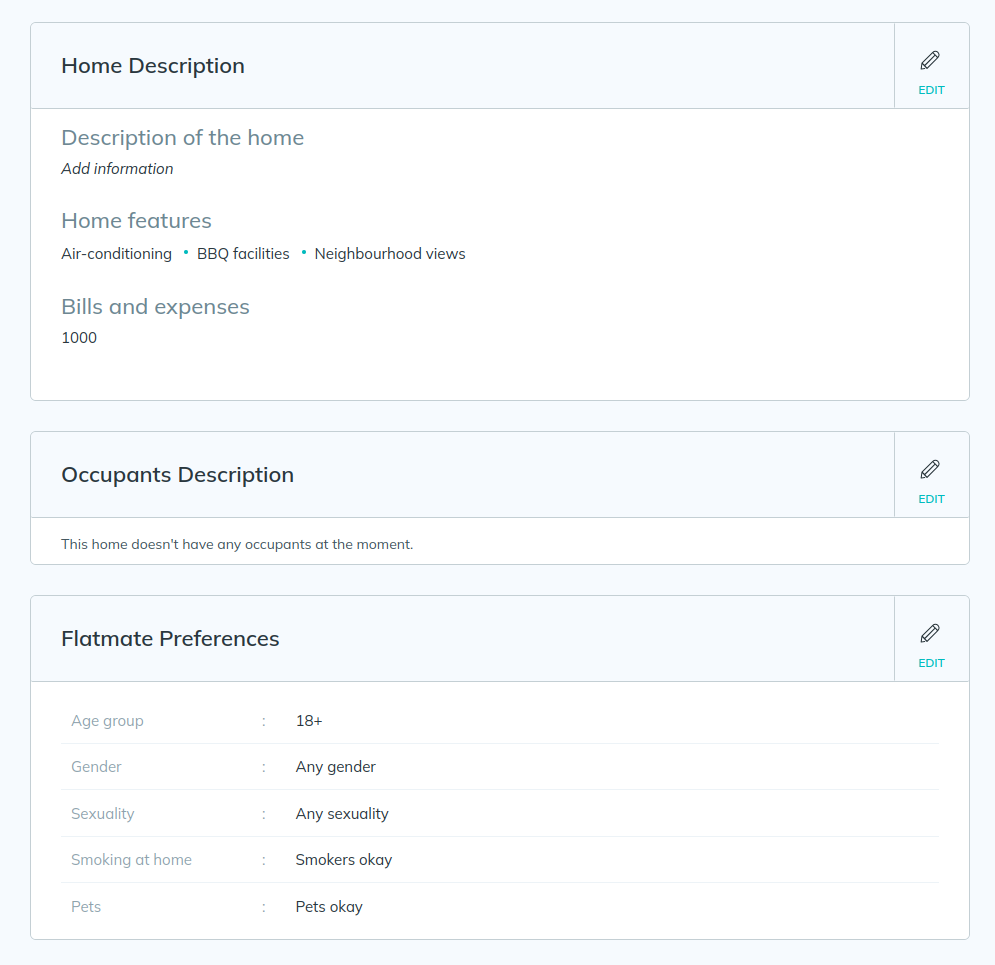
\includegraphics[width=0.8\textwidth]{fotos/home-flatmate.png}
    \caption{Configuración del perfil de la vivienda \textbf{}.}
\end{figure}
\subsubsection*{Interfaz y usabilidad}
La aplicación presenta una interfaz intuitiva con un buen tiempo de respuesta, la aplicación destaca por ser fácil de usar y ofrecer en todo momento información al usuario sobre las recomendaciones. Es de destacar que tanto la parte de ofertante como la de buscador tienen coherencia en cuanto a estilo y son muy personalizables.

\subsubsection*{Características destacadas}
\begin{itemize}
    \item  \textbf{Sistema de recomendación:} Utiliza un porcentaje de compatibilidad entre posible inquilino y vivienda, lo que facilita la búsqueda.
    \item \textbf{Explicación de compatibilidad:} Muestra un porcentaje indicando el grado de compatibilidad, además refleja las razones de incompatibilidad para dar "feedback" al usuario.
    \item \textbf{Configuración de perfil:} La creación de perfiles tanto para usuario como para propietario permite representar bien los intereses que se buscan en la comunidad o que tienen los usuario, siendo además sencillo y rápido de configurar. 
\end{itemize}
\begin{figure}[H]
    \centering
    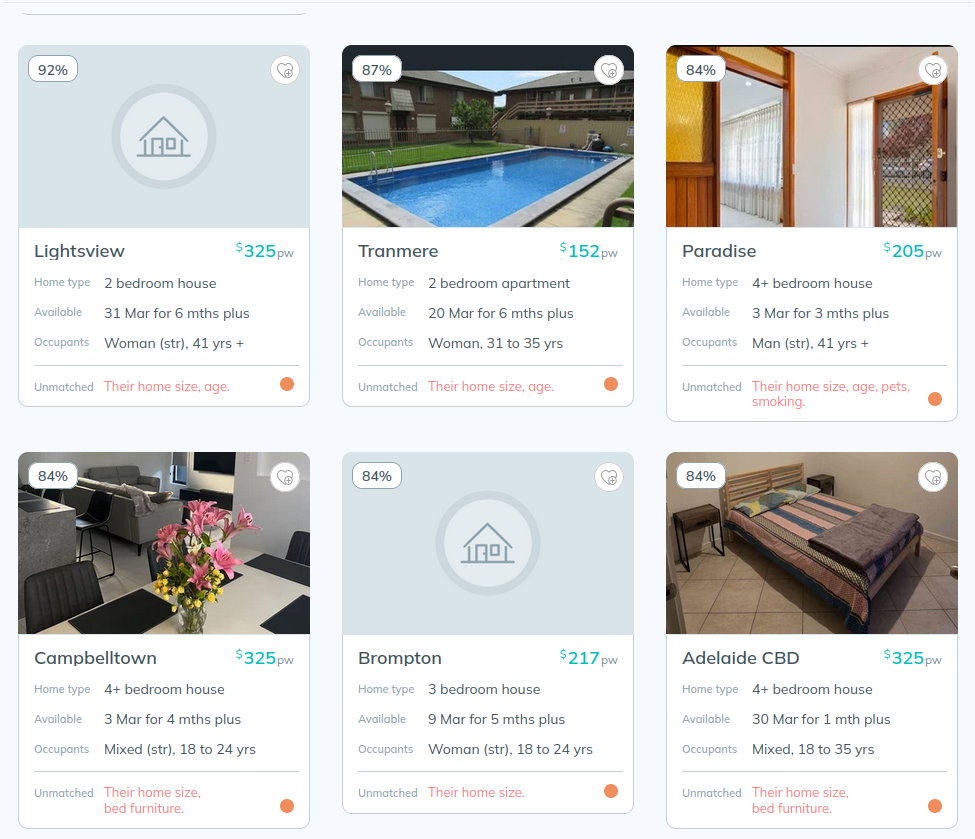
\includegraphics[width=1\textwidth]{fotos/flatmate-matches.png}
    \caption{Sección de búsqueda de vivienda por afinidad\textbf{}.}
\end{figure}
\subsubsection*{Limitaciones}
\begin{itemize}
    \item La aplicación únicamente está disponible en Australia, lo que limita enormemente su uso.
    \item No ofrece ningún tipo de herramienta para administrar las tareas de la vivienda una vez creado el piso compartido.
    \item La compatibilidad se basa en aspectos básicos como la edad, el género y si se es fumador, sin un análisis más profundo de la afinidad entre compañeros.
\end{itemize}

\subsubsection*{Conclusión}
Es una aplicación que ofrece una buena solución para buscar piso en función de afinidad, además el feedback que da al usuario con los porcentajes  e indicaciones sobre porque no coinciden son puntos muy favorables. Sin embargo, su única disponibilidad en Australia y la poca complejidad del algoritmo de recomendación provoca que no ofrezca una solución completa.

\subsection{Gestión de tareas en pisos compartidos}

\subsubsection{Flatify}
\emph{Flatify} \cite{Flatify} ofrece diversas funcionalidades enfocadas en la gestión de un piso compartido, entre las que destacan:
\begin{itemize}
    \item \textbf{Calendario compartido:} Permite añadir eventos para todos los integrantes.
    \item \textbf{Gestión de gastos:} Facilita el registro de pagos y el reparto de costes.
    \item \textbf{Lista de compras:} Los usuarios pueden añadir y marcar productos comprados.
    \item \textbf{Plan de limpieza:} Asigna tareas equitativamente entre los miembros del hogar.
    \item \textbf{Chat grupal:} Comunicación integrada para coordinarse fácilmente.
\end{itemize}

\begin{figure}[H]
    \centering
    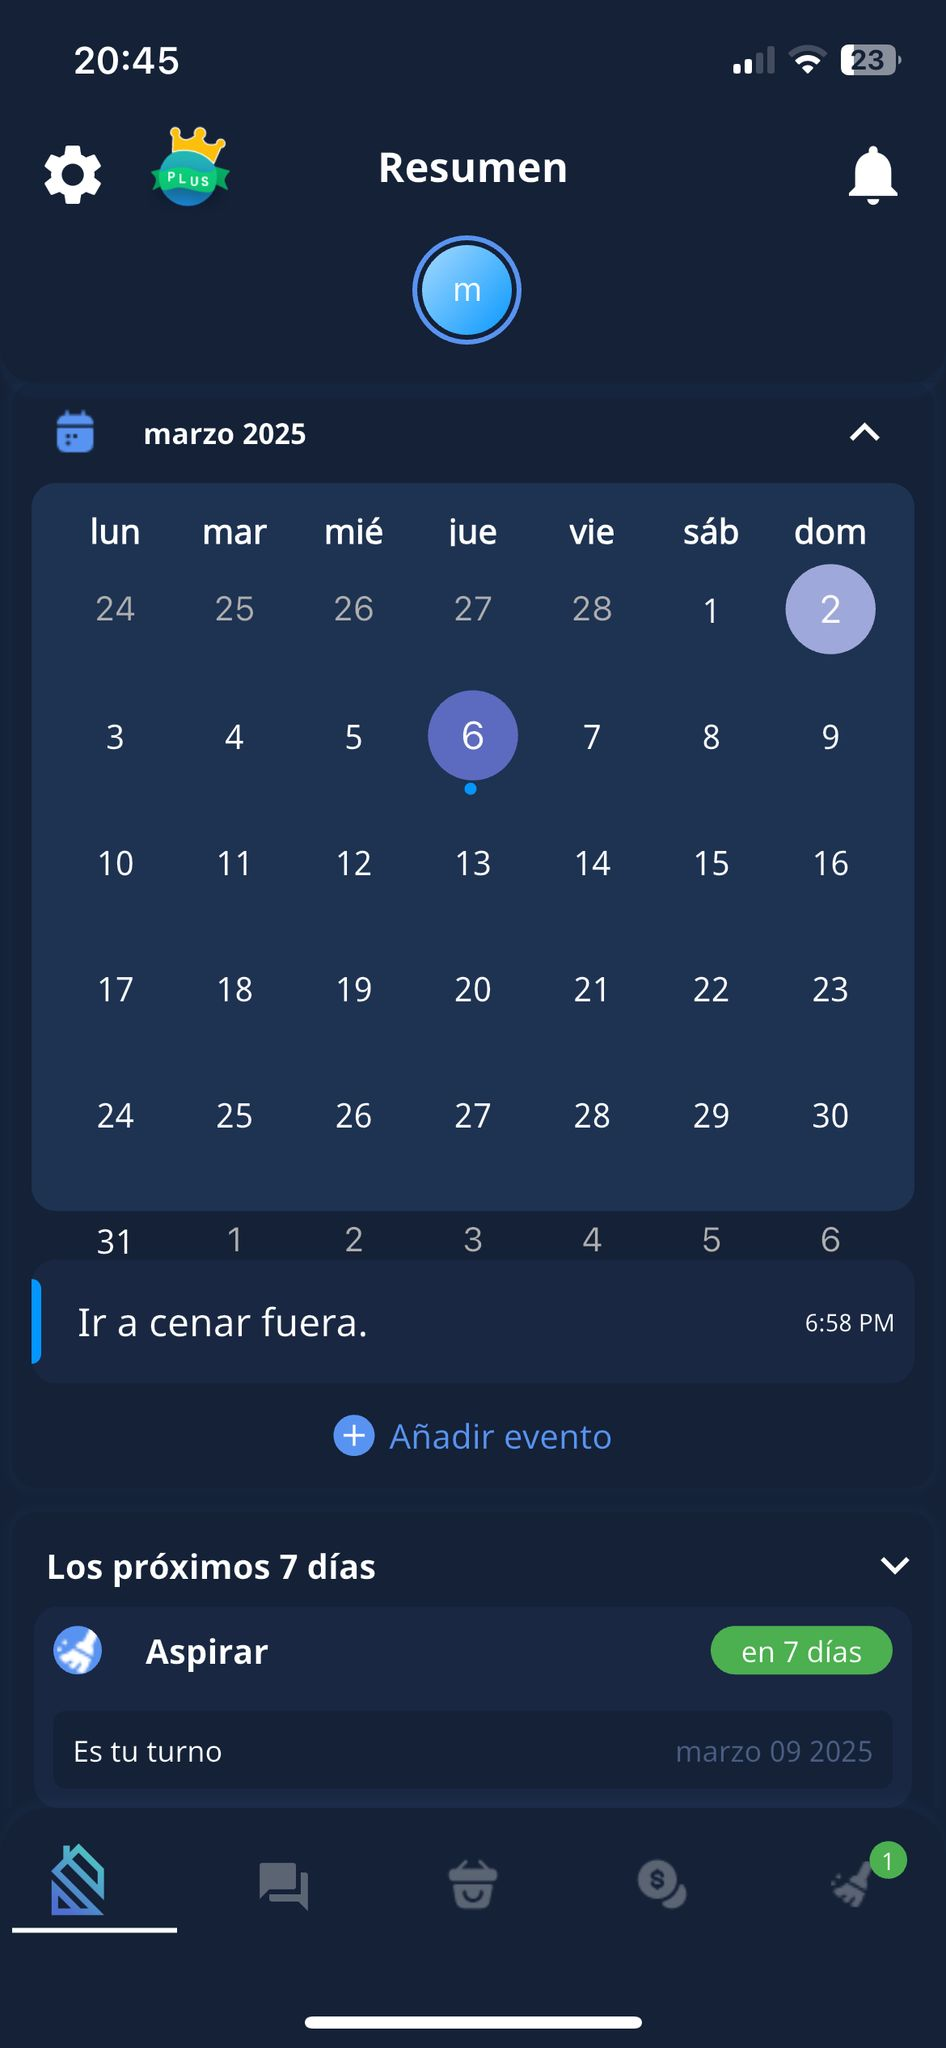
\includegraphics[width=0.4\textwidth]{fotos/Home-flatify.jpeg}
    \caption{Calendario de la aplicación\textbf{}.}
\end{figure}
\newpage
\subsubsection*{Interfaz y usabilidad}
La aplicación cuenta con una interfaz limpia e intuitiva, facilitando la navegación. Además, incluye una guía de primeros pasos útil para familiarizarse rápidamente con sus funciones.

\subsubsection*{Características destacadas}
\begin{itemize}
    \item \textbf{Distribución de tareas:} Permite establecer una secuencia de usuarios para rotar las responsabilidades de forma automática, asegurando una distribución justa.
    \item \textbf{Lista de compras:} Funciona correctamente, aunque la funcionalidad de subir facturas para gestionar los pagos está limitada a la versión premium.
    \item \textbf{Calendario:} Útil para eventos, pero no integra las tareas del hogar, lo que limita su funcionalidad.
\end{itemize}
\begin{figure}[H]
    \centering
    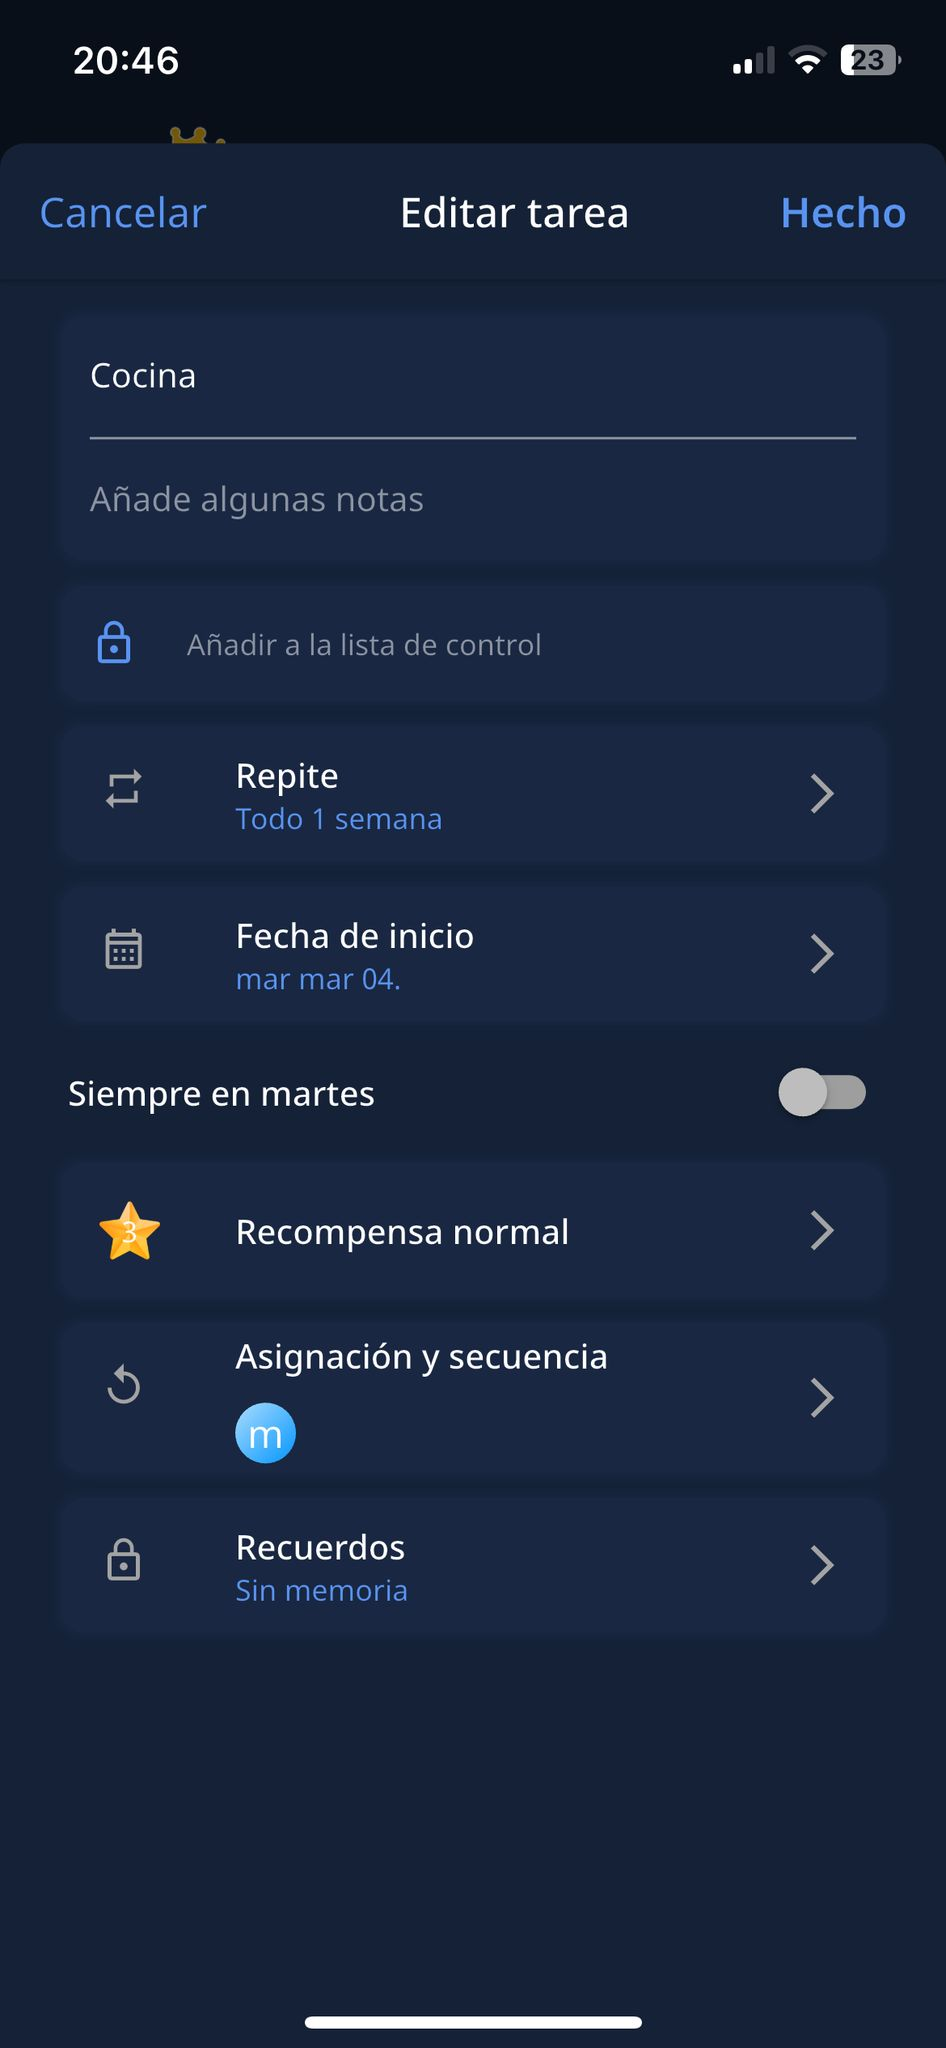
\includegraphics[width=0.4\textwidth]{fotos/creacion-tarea-flatify.jpeg}
    \caption{Sección para crear y editar una tarea\textbf{}.}
\end{figure}

\subsubsection*{Limitaciones}
\begin{itemize}
    \item Muchas características clave requieren pago o implican ver anuncios para su uso.
    \item La gestión de pagos y la lista de la compra no están bien sincronizadas, lo que reduce su utilidad.
    \item El calendario no permite gestionar tareas, desaprovechando su potencial.
\end{itemize}
\subsubsection*{Conclusión}
A pesar de las limitaciones de su versión gratuita, esta aplicación es la mejor solución encontrada para la gestión de pisos compartidos, ya que ofrece diversas herramientas útiles para la organización del hogar. Sin embargo, presenta algunos inconvenientes como una funcionalidad de calendario que resulta incompleta y la ausencia de herramientas para la creación de hogares basados en afinidades. Estas carencias hacen que la aplicación no sea una opción viable para nuestro problema.

\section{Tecnologías en el mercado}
Para el desarrollo del sistema será necesario apoyarse en diferentes tecnologías que permitan constuir un sistema que responda a las necesidades planteadas.
Con el actual auge del desarrollo software, numerosas tecnologías están apareciendo en el mercado para facilitar y mejorar la calidad del desarrollo. A continuación, se realiza un análisis de las tecnologías más relevantes y las ventajas que pueden ofrecer.

\begin{figure}[H]
    \centering
    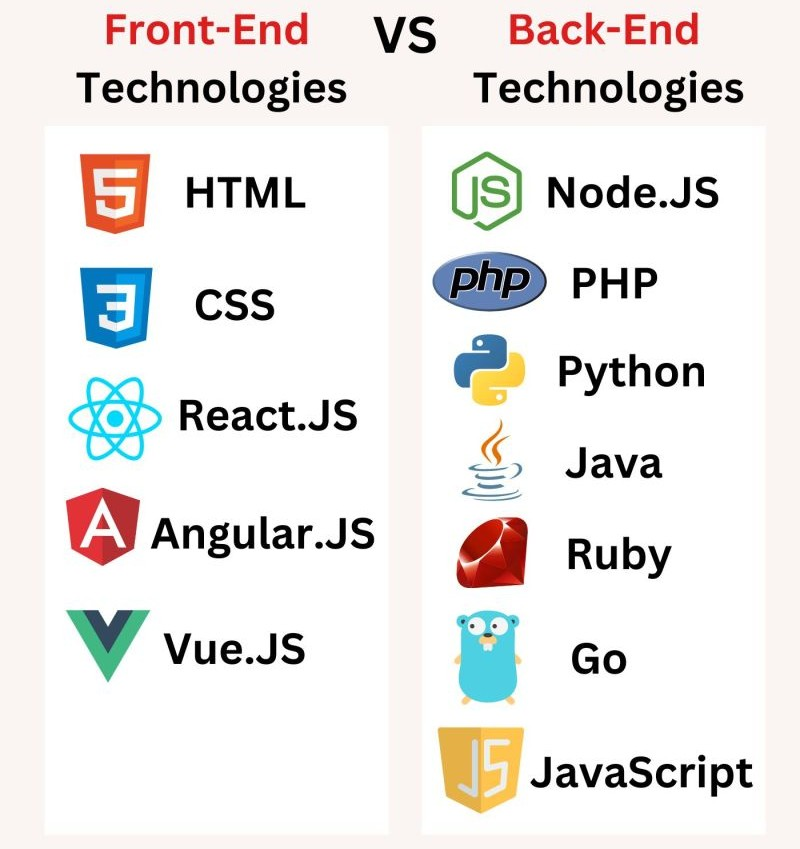
\includegraphics[width=0.45\textwidth]{fotos/lenguajes.jpg}
    \caption{Lenguajes de programación y tecnologías presentes en el mercado\textbf{}.}
    \label{fig:lenguajes-programacion}
\end{figure}
\subsection{Back-End}
\subsubsection*{Python-Django}
Con el aumento de popularidad de Python \cite{Top_Language_GitHub}, varios frameworks han aparecido para llevar su funcionamiento al Back-End, como se muestra en la imagen \ref{fig:lenguajes-programacion}. Entre ellos, destacan FastAPI, Django y Flask. Estos frameworks aprovechan las ventajas de Python, un lenguaje orientado a la legibilidad y popularizado por el auge de la inteligencia artificial. Django es el más destacable por su robustez y numerosas utilidades. Aunque FastAPI y Flask son excelentes para desarrollar APIs por ser ligeros y especializados, siendo más adecuados para aplicaciones menores, mientras que Django cubre aplicaciones complejas que requieren escalabilidad o seguridad a partir del uso del patrón MVC \cite{MVC}.

\subsubsection*{NodeJS- Express}
NodeJS\cite{NodeJS} ha revolucionado el desarrollo Back-End al permitir la ejecución de código JavaScript en el lado del servidor, facilitando así la unificación de tecnologías utilizadas tanto en el Front-End como en el Back-End, como muestra la imagen \ref{fig:lenguajes-programacion}, con tecnologías como React en el Front-End y NodeJS en el Back-End. Entre sus características principales se encuentra su gestión de la asincronía mediante un modelo no bloqueante que utiliza un ``event loop``, lo cual permite procesar solicitudes sin bloquear el hilo principal, tal como se muestra en la Figura \ref{fig:nodejs}. Además, ofrece facilidad para trabajar con objetos JavaScript similares a JSON y ha dado lugar a la aparición de frameworks que lo complementan; en este caso, nos centraremos en Express, que facilita la gestión de rutas y la creación de aplicaciones web escalables.
\begin{figure}[H]
    \centering
    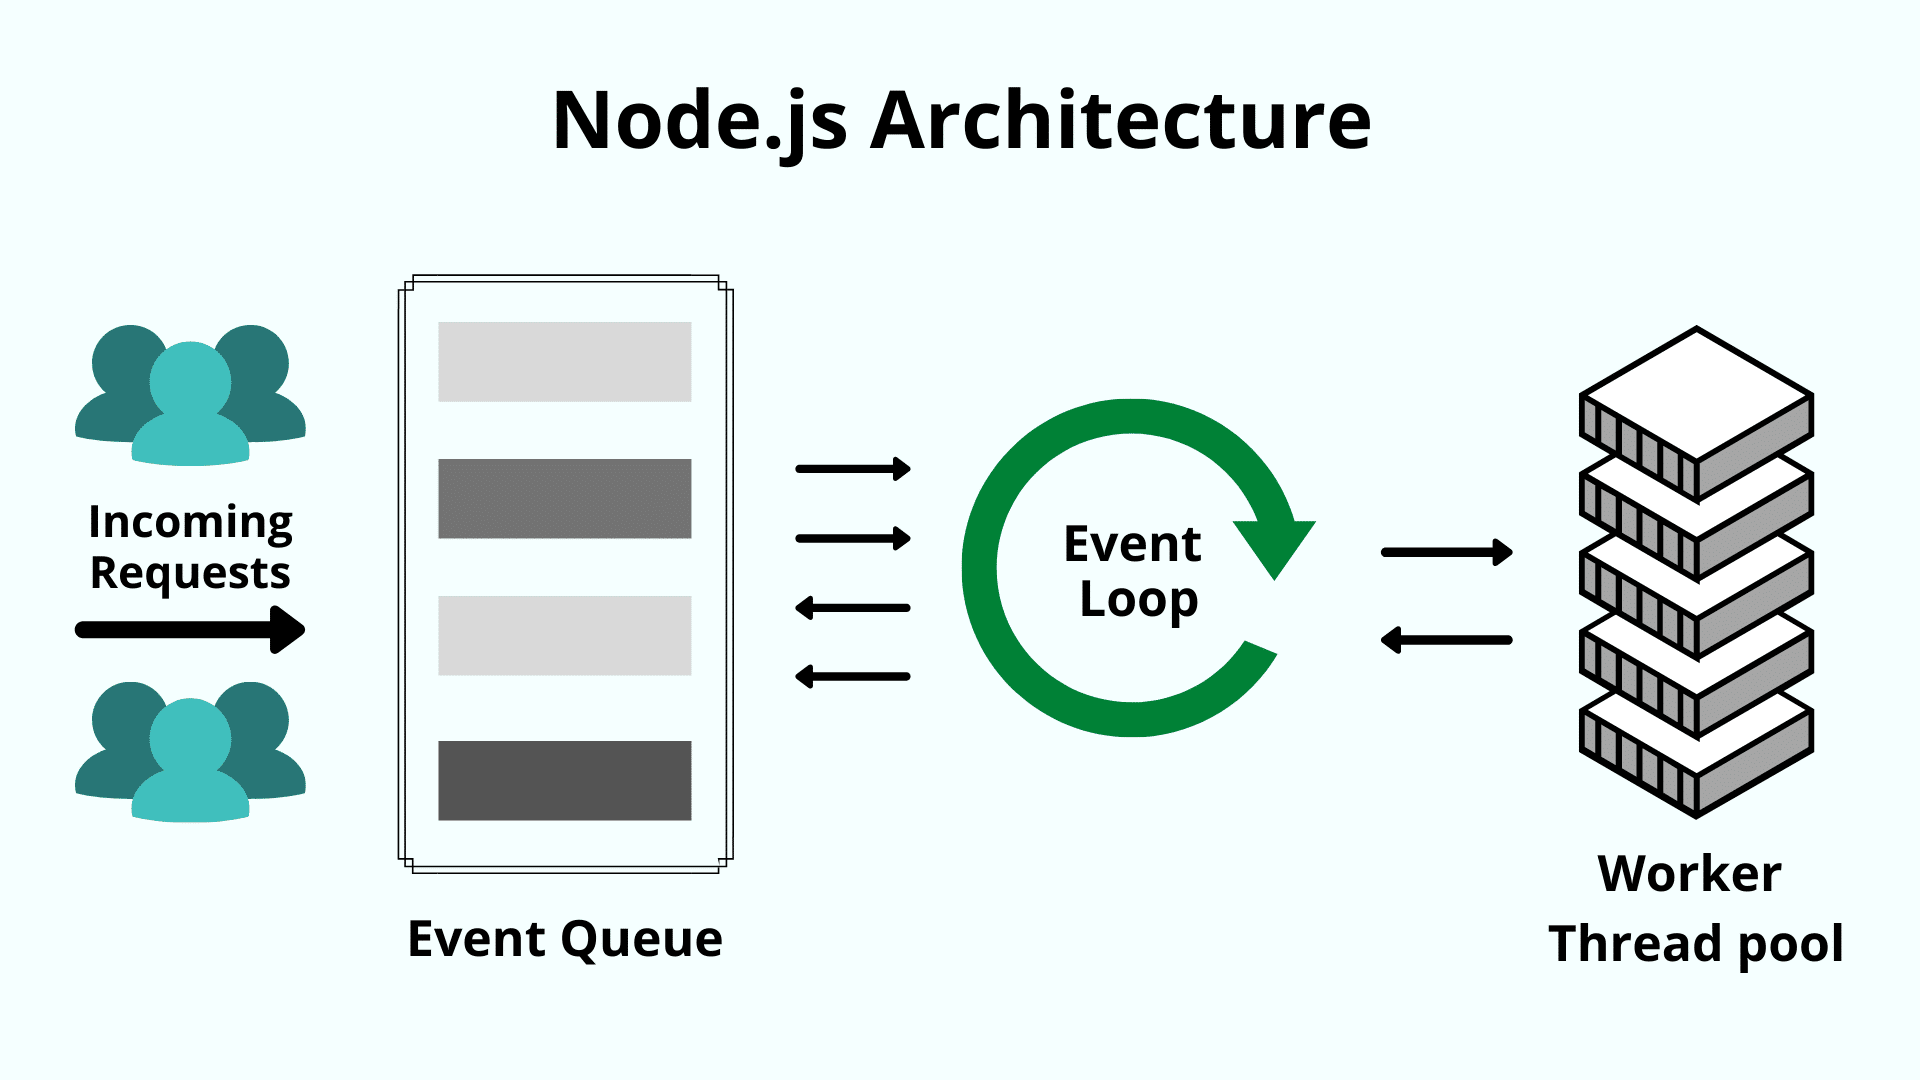
\includegraphics[width=1\textwidth]{fotos/node-js2.png}
    \caption{Arquitectura NodeJS\textbf{}.}
    \label{fig:nodejs}
\end{figure}
\subsubsection*{Java}
Java, conocido por su fuerte tipado y su compilación, ofrece una solución robusta para el desarrollo Back-End con Spring Boot. Este framework simplifica la gestión de dependencias, proporcionando una estructura más fácil de manejar que la versión anterior de Spring. Es ampliamente utilizado en entornos empresariales debido a su capacidad para soportar arquitecturas complejas, como microservicios o arquitectura hexagonal. Además, Spring Boot promueve prácticas avanzadas de desarrollo como la inyección de dependencias y sus starters, los cuales se pueden apreciar en la imagen \ref{fig:spring}, incluyen desde seguridad hasta manejo reactivo de peticiones. Es una opción robusta para aplicaciones a gran escala. 
\begin{figure}[H]
    \centering
    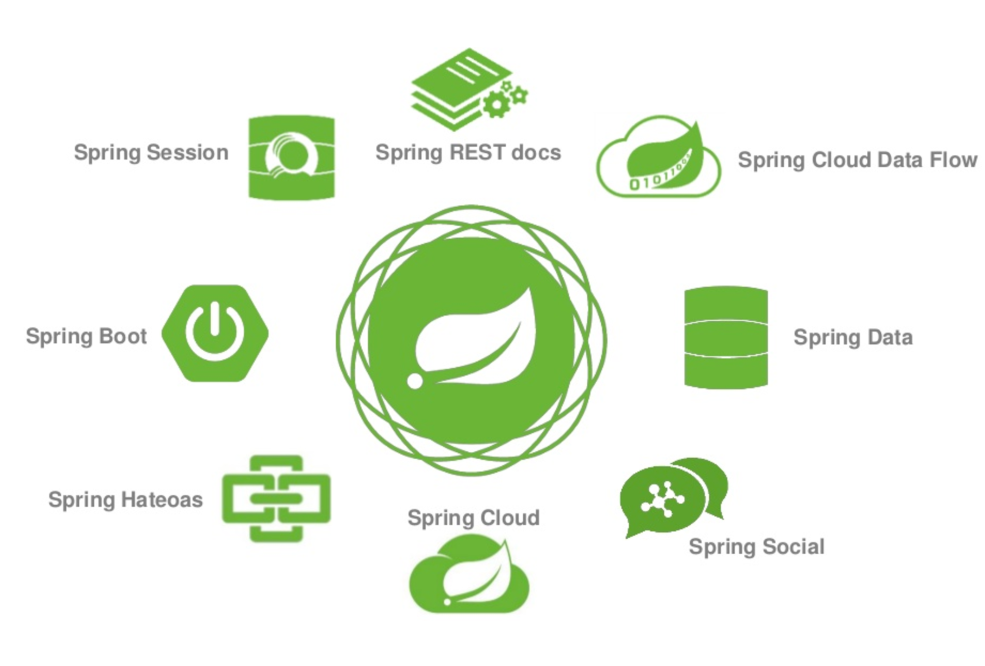
\includegraphics[width=0.8\textwidth]{fotos/tete.png}
    \caption{Starters de Spring Boot\textbf{}.}
    \label{fig:spring}
\end{figure}
\subsection{Front-End}
En el desarrollo Front-End, JavaScript se ha consolidado como el estándar principilar con la aparición de numerosos frameworks. A continuación se van a analizar las opciones más interesantes para la parte visual de la aplicación.
\subsubsection*{React}
React es en la actualidad la biblioteca de desarrollo Front-End más demandada \cite{Frontend_Frameworks_DevJobsScanner}. Su enfoque basado en la creación de componentes reutilizables, el uso de JSX que permite escribir código similar a HTML dentro de archivos JavaScript, como se puede observar en la imagen \ref{fig:react}, junto con la gestión de estados y hooks,  permite estructurar aplicaciones de manera escalable y eficiente de forma sencilla. Además su amplica adopción y su extensa comunidad y documentación lo convierten en una gran herramienta a la hora de crear interfaces complejas y dinámicas.
\begin{figure}[H]
    \centering
    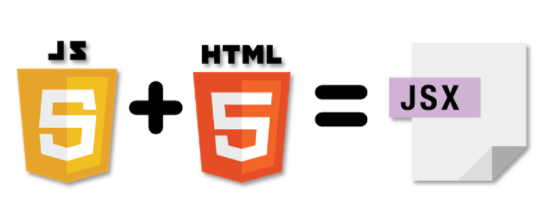
\includegraphics[width=0.8\textwidth]{fotos/react.PNG}
    \caption{Explicación del concepto JSX\textbf{}.}
    \label{fig:react}
\end{figure}
\subsubsection*{Angular}
Angular es un framework más completo y estructurado en comparación con React, que se centra más en ofrecer al usuario herramientas listas para usar. Sigue también el concepto de componentes pero con un enfoque más estricto en cuanto a arquitectura y estructura del proyecto, lo cual ayuda en la creación de aplicaciones robustas y mantenibles.

\subsubsection*{TypeScript}
El notable crecimiento en la popularidad de TypeScript se debe a que proporciona un sistema de tipado estático sobre JavaScript, lo cual ayuda a reducir errores en tiempo de compilación y mejora la detección de errores y legibilidad del código como se muestra en la imagen \ref{fig:ts}. TypeScript se está convirtiendo en un estándar dentro del desarrollo Front-End profesional debido a la gran ayuda que ofrece para detectar de forma temprana errores y su integración con cualquier tipo de framework moderno como React y Angular.
\begin{figure}[H]
    \centering
    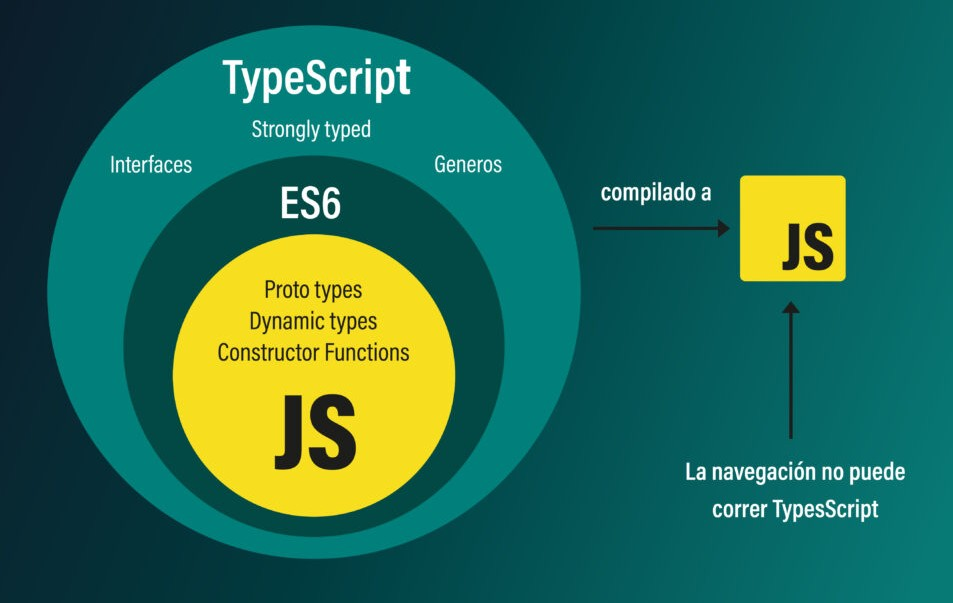
\includegraphics[width=0.8\textwidth]{fotos/typescript.jpg}
    \caption{Explicación del concepto de TypeScript\textbf{}.}
    \label{fig:ts}
\end{figure}

\subsection{Base de Datos}
\begin{figure}[H]
    \centering
    
\includegraphics[width=0.3\textwidth]{fotos/postgre.png}
    \caption{Logo PostgreSQL\textbf{}.}
    \label{fig:psql}
\end{figure}
\subsubsection*{PostgreSQL}
PostgreSQL \ref{fig:psql} es una base de datos relacional \textit{open source} que se destaca por su alto rendimiento, escalabilidad y fiabilidad. Garantiza transacciones \textit{ACID} (Atomicidad, Consistencia, Aislamiento y Durabilidad) \cite{cics-acid}, lo que asegura que las operaciones en la base de datos se realicen de forma segura y consistente. Además, PostgreSQL ofrece una robusta seguridad y es respaldada por una comunidad activa que mantiene una documentación extensa y detallada.
\begin{figure}[H]
    \centering
    
\includegraphics[width=0.5\textwidth]{fotos/mongo.png}
    \caption{Logo MongoDB\textbf{}.}
    \label{fig:mongo}
\end{figure}
\subsubsection*{MongoDB}
MongoDB \ref{fig:mongo} es una base de datos no relacional que almacena los datos en formato BSON (Binary JSON), lo que le permite manejar grandes volúmenes de datos de manera eficiente. Se caracteriza por su alto rendimiento, flexibilidad y facilidad para integrarse con aplicaciones modernas. A diferencia de las bases de datos relacionales, MongoDB no requiere esquemas estrictos, lo que lo hace ideal para manejar datos no estructurados o semi-estructurados, facilitando la evolución y adaptación de los modelos de datos.

\section{Conclusión tras estudiar el mercado}
Tras analizar diversas alternativas disponibles en el mercado, hemos identificado aplicaciones que abordan parcialmente la problemática planteada. \textit{Flatmate Finders} facilita la búsqueda de compañeros de piso en función de la afinidad, mientras que \textit{Flatify} destaca en la gestión de la convivencia, ofreciendo herramientas para la organización de tareas, calendario compartido y lista de la compra.

Sin embargo, ninguna de estas soluciones integra ambas funcionalidades en una única plataforma. La falta de una aplicación que combine tanto la búsqueda de vivienda como su gestión diaria con todos los requisitos necesarios, evidencia la necesidad de desarrollar este proyecto, ofreciendo una solución integral que cubra todas las necesidades de la vida en pisos compartidos basado en el \emph{co-housing}. En cuanto a las tecnologías todas las comentadas cumplen con los requisitos mínimos de funcionalidad para poder llevar a cabo el proyecto, por tanto la tecnología escogida dependerá de la arquitectura, preferencia del equipo de desarrollo y complejidad de la aplicación.
